\title{CS534 Implementation Assignment 2:\\Naive Bayes}
\author{
        Amit Bawaskar, Michael Lam\\
        EECS, Oregon State University\\
        %\email{}
        %\and
}

\documentclass[12pt]{article}
\usepackage[english]{babel}
\usepackage{graphicx}
\usepackage{subfig}
\usepackage{amsmath}
\usepackage{hyperref}
\hypersetup{
    colorlinks,%
    citecolor=green,%
    filecolor=magenta,%
    linkcolor=red,%
    urlcolor=cyan
}

%\underset{x}{\operatorname{argmax}}
%\underset{x}{\operatorname{argmin}}
\DeclareMathOperator*{\argmin}{arg\,min}
\DeclareMathOperator*{\argmax}{arg\,max}

\begin{document}
\maketitle

\begin{abstract}
In this assignment, we implemented the Naive Bayes classifier with the Bernoulli model and Multinomial model, and compared their performance.
\end{abstract}

% -------------------------------------------------
\section{Introduction}
We implemented the Naive Bayes classifier to solve a document classification problem on the 20-newsgroup data set. Two models were implemented and compared for performance: Bernoulli model and Multinomial model.

\section{Naive Bayes}
Paragraph about Naive Bayes.

\subsection{Model}
Naive Bayes assumes that the features are independent.

\subsection{Inference}
Inference is performed by using Bayes rule with the learned likelihood and prior probabilities, and using decision theory to select the class that maximizes the posterior probability.

\subsection{Learning}
Learning the likelihood probabilities for each feature and class is done by maximum a posteriori estimation. Equivalently this amounts to applying Laplace smoothing to the maximum likelihood estimator. The prior probabilities for each class is the maximum likelihood estimator for it.

\subsection{Implementation Details}
In this project we operated with the log of probabilities in order to avoid underflow issues. That is, for every multiplication and division operation, we instead used addition and subtraction of the log of the operands. We also stored the log of probabilities. For decision theory, we simply selected the class that maximizes the log of the posterior probability since the log function is a monotonically increasing function. Thus we operated with the log of probabilities for every circumstance.

We also applied Laplace smoothing to the likelihood probability of each feature and class in order to assign a default prior to words that have not been encountered.

\section{Bernoulli Model}
Paragraph about Bernoulli model.

The overall test accuracy for the Bernoulli model is \textbf{0.772152}. Figure \ref{fig:confusionmat_bern} shows the confusion matrix.

\begin{figure}[!t]
  \centering
  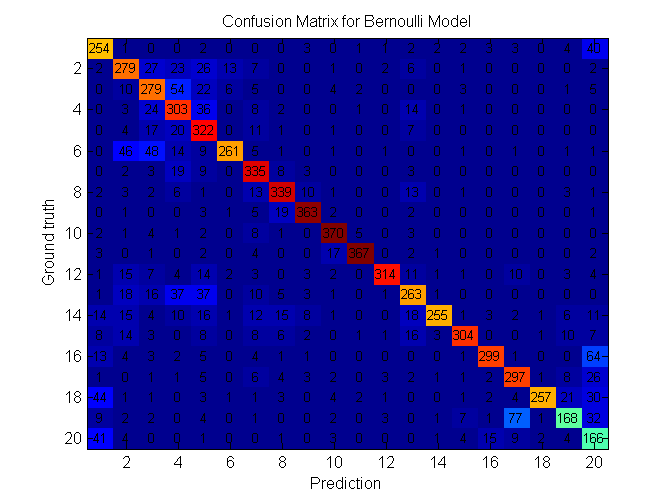
\includegraphics[scale=1]{img/confusionmat_bern.png}
  \caption{Confusion matrix for the Bernoulli model.}
  \label{fig:confusionmat_bern}
\end{figure}

\section{Multinomial Model}

Paragraph about Multinomial model.

Report overall testing accuracy.

Report the confusion matrix.

%Figure \ref{fig:examplefigure} is an example.
%
%\begin{figure}[!t]
%  \centering
%  \includegraphics[scale=.70]{img/path_to_image.png}
%  \caption{Caption here}
%  \label{fig:examplefigure}
%\end{figure}

\section{Heuristics for Reducing Vocabulary Size}

We explored several heuristic strategies for reducing the vocabulary size in hopes of improving classification accuracy.

We tried eliminating words in the dictionary that have length less than  or equal to a certain threshold value. We explored thresholds from 0 to 5, meaning keeping all words to keeping only words with length greater than 5. The results in Figure \ref{fig:vocabthreshold} indicate that the classification accuracy increased negligibly when eliminating words up to 2 letters long, but decreased noticeably as the threshold increases after 2 letters.

\begin{figure}[!t]
  \centering
  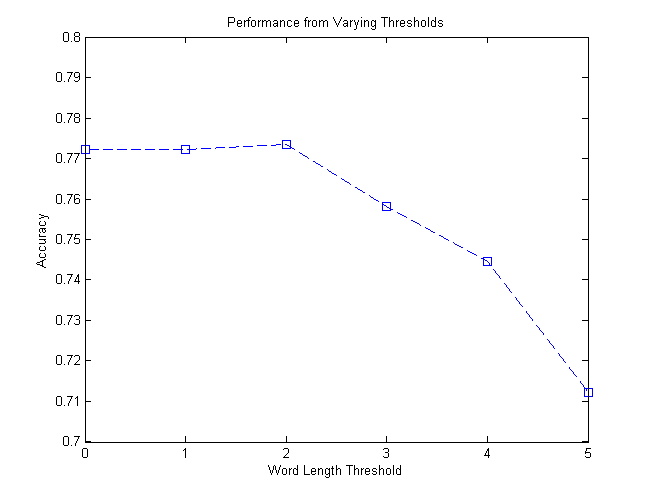
\includegraphics[scale=.70]{img/vocabthreshold.png}
  \caption{Classification accuracy using the Bernoulli model and varying word length thresholds. Words of length less than or equal to the threshold value are omitted in the vocabulary for learning and inference.}
  \label{fig:vocabthreshold}
\end{figure}

\end{document}
This is never printed
